\section{Our Approach}

A precise solution to the monitoring problem at hand would include considering all interleavings of the concurrent events in the given distributed signal.
The partial synchrony assumption helps reduce the number of such interleaving, however, the state-of-the-art leveraging this assumption relies on off-the-shelf SMT solvers and thus are not able to provide theoretical guarantees on running time and memory consumption~\cite{GangulyMB20,MomtazAB23}.
In order to design a dedicated monitoring algorithm with provable guarantees, we introduce the bounded variability assumption and an inexpensive method to overapproximate the set of behaviors of the distributed signal.
We assume a central monitor that knows the values of $\varepsilon$ and $\delta$ as well as the initial values of the signals.

%TODO: add a short paragraph explaining each subsection

\subsection{Uncertainty Regions and Canonical Segmentations} \label{sec:segment}

Consider a signal $x : [0,d) \to \R$ with a single rising edge from value 2 to 3 at local time $t$.
The monitor observing this signal needs to take into account how the local clock of the agent producing $x$ relates with the global clock: due to clock skew, the rising edge of $x$ occurs in the range $(t - \varepsilon, t + \varepsilon)$ according to the global clock.
This range is called an \emph{uncertainty region} because in the interval $(t - \varepsilon, t + \varepsilon)$ the monitor cannot tell the value of $x$ precisely, but only that it changes from 2 to 3.
To systematically reason about uncertainty regions of signals, we use the notion of segmentation of temporal domains of signals.

Given a temporal domain $I = [0,d) \subset \R_{\geq 0}$, a \emph{segmentation} of $I$ is a partition of $I$ into finitely many intervals $I_1, \ldots, I_k$ of the form $I_j = [t_j, t_{j+1})$ such that $t_j < t_{j+1}$ for all $1 \leq j \leq k$.
By extension, a segmentation of a collection of signals with the same temporal domain $I$ is a segmentation of $I$.

Let $x : [0,d) \to \R$ be a signal and $D_x = \{(t_1, x(t_1)), \ldots, (t_m, x(t_m))\}$ be the set of edges of $x$, given in an increasing order of local clock values.
For $1 \leq i \leq m$, we let 
\begin{align*}
	\theta_{\text{lo}}(x,t_i) &= \max\{0, \max_{j \in \{1, i\}} t_j - \varepsilon - (j-i)\delta\} \text{, and} \\
	\theta_{\text{hi}}(x,t_i) &= \min_{i \leq j \leq m} t_j + \varepsilon - (j-i)\delta.
\end{align*}
Intuitively, $\theta_{\text{lo}}$ and $\theta_{\text{hi}}$ give us the lower and upper bounds on the value of the global clock for a given edge, i.e., the bounds on the uncertainty region of the edge.
We use these to describe a canonical segmentation of a distributed signal.

Let $(S,{\hb})$ be a distributed signal of $n$ signals.
For each signal $x_i$, let $F_i = \{\theta_{\text{lo}}(x_i, t_j) \st (t_j, x_i(t_j)) \in D_{x_i}\} \cup \{\theta_{\text{hi}}(x_i, t_j) \st (t_j, x_i(t_j)) \in D_{x_i}\}$ be the set of bounds on its uncertainty regions.
Let $d' = \max(d, \max (\bigcup_{i = 1}^{n} F_i))$, which corresponds to the duration of the distributed signal with respect to the global clock.
We define $F_S = \{0, d'\} \cup \bigcup_{i = 1}^{n} F_i$ and let $(a_j)_{1 \leq j \leq |F|}$ be an increasing sequence of clock values corresponding to the elements of $F$.
We define the \emph{canonical segmentation} of $(S,{\hb})$ as $G_S = \{I_1, \ldots, I_{|F| - 1}\}$ where $I_j = [a_j, a_{j+1})$ for all $1 \leq j < |F|$.

\begin{example} \label{ex:canonseg}
	Let $(S, {\hb})$ be a distributed signal with $S = (x_1, x_2)$ over the temporal domain $[0,8)$ such that $\pi(x_1) \neq \pi(x_2)$.
	Suppose $x_1(0) = 0$ and $x_2(0) = 1$ and let $\varepsilon = 2$ and $\delta = 3$.	
	Consider the case where $x_1$ has a rising edge $(3,1)$ and a falling edge $(5,0)$ while $x_2$ only has a falling edge $(4,0)$.
	For $x_1$, taking into account only the clock skew would give us the uncertainty regions $(1,5)$ and $(3,7)$.
	However, the computation of uncertainty regions take into account also the bounded variability.
	Intuitively, if the rising edge of $x_1$ occurs at global time 1, considering bounded variability, its falling edge occurs at the earliest at global time 4 instead of 3.
	Conversely, if the falling edge occurs at global time 7 then its rising edge occurs at the latest at global time 4 instead of 5.
	Then, we obtain $F_1 = \{1, 4, 7\}$ and $F_2 = \{2, 6\}$, therefore $F_S = \{0, 1, 2, 4, 6, 7, 8\}$.
	This leads to the canonical segmentation $G_S = \{[0,1), [1,2) ,[2,4) ,[4,6) ,[6,7) ,[7,8)\}$.		
\end{example}

\subsection{Value Expressions}
In uncertainty regions, although the monitor is not able to determine the exact value of a signal at a time point, it knows how the signal values change.
To capture this information, we use short sequences of possible signal values capturing how a signal behaves within a segment and several operations on them to propagate the information from real-valued signals to truth values subformulas.

Let $\Sigma$ be a finite alphabet corresponding to a set of signal values.
A \emph{value expression} is a finite word in $\destutter(\Sigma^*)$.
Given $m \geq 2$ and value expressions $u_1, \ldots, u_m$, we define their \emph{asynchronous product} to encode their potential interleavings as follows:
\small
$$u_1 \otimes \ldots \otimes u_m = \left\lbrace  \destutter(v_1, \ldots, v_m) \st \max_{1 \leq i \leq m} |u_i| \leq k \leq \sum_{i = 1}^{m} |u_i|, v_i \in \stutter_k(u_i) \text{ for all } 1 \leq i \leq m \right\rbrace$$  
\normalsize
By extension, given $L_1, \ldots L_m \subseteq \destutter(\Sigma^*$), we have $L_1 \otimes \ldots \otimes L_m = \{ u_1 \otimes \ldots \otimes u_m \st u_i \in L_i \text{ for all } 1 \leq i \leq m\}$.

For $u_1, \ldots, u_m$ and a function $f : \Sigma^m \to \R$, we refer to the set of value expressions that can be obtained by applying $f$ to their asynchronous product as follows: $f(u_1, \ldots, u_m) = \destutter(\{(f(v_1[i], \ldots, v_m[i]))_{1 \leq i \leq |v_1|} \st (v_1, \ldots, v_m) \in u_1 \otimes \ldots \otimes u_m\})$.
Moreover, for $c \in \R$, we write $f(u_1, \ldots, u_m) > c$ to denote the set $\destutter(\{(f(v_1[i], \ldots, v_m[i]) > c)_{1 \leq i \leq |v_1|} \st (v_1, \ldots, v_m) \in u_1 \otimes \ldots \otimes u_m\})$ where $f(v_1[i], \ldots, v_m[i]) > c$ is 1 if the inequality holds, and it is 0 otherwise.

\begin{example} \label{ex:valexpr}
	Let $\Sigma = \{2, 3, 5, 7\}$ and consider the value expressions $u_1 = 2 \cdot 5$ and $u_2 = 3 \cdot 7$.
	These expressions respectively model the behaviors of potentially asynchronous signals whose values change from 2 to 5 and from 3 to 7.
	To compute their asynchronous product, we range the stuttering from $k = 2$ to $k = 4$.
	For $k = 2$, we obtain the tuple $(2 \cdot 5, 3 \cdot 7)$.
	For $k = 3$, stuttering $u_1$ leads to $2 \cdot 2 \cdot 5$ or $2 \cdot 5 \cdot 5$ while stuttering $u_2$ gives us $3 \cdot 3 \cdot 7$ or $3 \cdot 7 \cdot 7$.
	Putting them together, we get the new tuples $(2 \cdot 2 \cdot 5, 3 \cdot 7 \cdot 7)$ and $(2 \cdot 5 \cdot 5, 3 \cdot 3 \cdot 7)$ while the others yield $(2 \cdot 5, 3 \cdot 7)$ once destuttered, which we obtained earlier.
	For $k = 4$, all the tuples coincide with the earlier ones once destuttered.
	Intuitively, $(2 \cdot 5, 3 \cdot 7)$ captures the case when the rising edges of the corresponding signals occur simultaneously.
	Similarly, $(2 \cdot 2 \cdot 5, 3 \cdot 7 \cdot 7)$ corresponds to the edge of $u_2$ happening before that of $u_1$, and $(2 \cdot 5 \cdot 5, 3 \cdot 3 \cdot 7)$ vice versa.
	
	Now, to compute the function $u_2 - u_1$ we apply the function letter by letter to the tuples in their asynchronous product.
	For example, applying it to $(2 \cdot 5, 3 \cdot 7)$ results in $(3 - 2) \cdot (7 - 5)$, and thus $v_1 = 1 \cdot 2$.
	Similarly, we get $v_2 = 1 \cdot 5 \cdot 2$ and $v_3 = 1 \cdot -2 \cdot 2$ from the rest.
	Finally, if we take the constraint that $u_2 - u_1  > 0$, the expressions $v_1$ and $v_2$ coincide after destuttering and result in $1$, while $v_3$ gives us $1 \cdot 0 \cdot 1$.
\end{example}

As we will detail in the next section, after computing the value expressions of real-valued signals, we compute those of satisfaction signals of atomic propositions and use these boolean value expressions in the evaluation of the STL formula.
Therefore, we assume a binary alphabet in the sequel.

Let $\Sigma = \{0,1\}$.
Given $u,v \in \Sigma^*$ of the same length, we respectively denote by $u \BitAnd v$ the bitwise-and operation, and by $\BitNeg u$ the bitwise-negation operation.
In addition, given nonempty words $u,v \in \Sigma^*$ of length $\ell$, we define auxiliary bitwise-temporal operators as follows:
\begin{align*}
\mathsf{E} u &= \left( \max_{i \leq j \leq \ell} u[j] \right)_{1 \leq i \leq \ell} \\
\mathsf{A} u &= \left( \min_{i \leq j \leq \ell} u[j] \right)_{1 \leq i \leq \ell} \\
u \mathsf{U}^0 v &= \left( \max_{i \leq j \leq \ell} \left( \min \left( v[j], \min_{i \leq k \leq j} u[k] \right) \right) \right)_{1 \leq i \leq \ell} \\
u \mathsf{U}^1 v &= \left( \max \left( u[i..] \mathsf{U}^0 v[i..], \mathsf{A} u[i..] \right) \right)_{1 \leq i \leq \ell} \\
\end{align*}
Note that the operators $\mathsf{E}$ and $\mathsf{A}$ respectively correspond to the \emph{eventually} and the \emph{always} operators of temporal logics.
Moreover, $\mathsf{U}^0$ corresponds to the standard (strong) \emph{until} operator while $\mathsf{U}^1$ is the \emph{weak until}.
As usual, $\mathsf{A} u = u \mathsf{U}^1 0^\ell$ and $\mathsf{E} u = 1^\ell \mathsf{U}^0 u$.
This distinction will be useful later when we evaluate value expressions segment by segment.

Below we use finite words from $\destutter(\Sigma^*)$ to denote how the values of a satisfaction signal evolve through intervals that include uncertainty and interleavings.
We use the following grammar to encode such expressions.
$$ \psi := 0 ~|~ 1 ~|~ \lnot \psi  ~|~ \psi \sqcap \psi ~|~ \psi \cdot \psi ~|~ \psi \until^0 \psi ~|~ \psi \until^1 \psi $$ %~|~ \psi + \psi   ~|~ \LTLf \psi ~|~ \LTLg \psi $$  %~|~ \psi \triangleleft \psi ~|~ \psi \triangleright \psi ~|~ \psi \diamond \psi

We denote by $\Psi$ the set of all expressions generated by the above grammar.
Letting $\psi_1, \psi_2 \in \Psi$, we inductively define the semantics for our encoding.
\begin{align*}
		\llbracket 0 \rrbracket &=  \{ 0 \} \\
		\llbracket 1 \rrbracket &=  \{ 1 \} \\
		\llbracket \lnot \psi_1 \rrbracket &= \{ \BitNeg u \st u \in \llbracket \psi_1 \rrbracket \} \\
%		\llbracket \psi_1 + \psi_2 \rrbracket &= \llbracket \psi_1 \rrbracket \cup \llbracket \psi_2 \rrbracket \\
		\llbracket \psi_1 \sqcap \psi_2 \rrbracket &= \destutter(\{ v_1 \BitAnd v_2 \st (v_1,v_2) \in \llbracket \psi_1 \rrbracket \otimes \llbracket \psi_2 \rrbracket \}) \\
		\llbracket \psi_1 \cdot \psi_2 \rrbracket &= \destutter(\{ u_1 u_2 \st u_1 \in \llbracket \psi_1 \rrbracket, u_2 \in \llbracket \psi_2 \rrbracket \}) \\
		\llbracket \psi_1 \until^0 \psi_2 \rrbracket &= \destutter(\{ v_1 \mathsf{U}^0 v_2  \st (v_1,v_2) \in \llbracket \psi_1 \rrbracket \otimes \llbracket \psi_2 \rrbracket \}) \\
		\llbracket \psi_1 \until^1 \psi_2 \rrbracket &= \destutter(\{ v_1 \mathsf{U}^1 v_2  \st (v_1,v_2) \in \llbracket \psi_1 \rrbracket \otimes \llbracket \psi_2 \rrbracket \}) \\
%		\llbracket \LTLf \psi \rrbracket &= \destutter(\{ \mathsf{E} u \st u \in \llbracket \psi \rrbracket \}) \\
%		\llbracket \LTLg \psi \rrbracket &= \destutter(\{ \mathsf{A} u \st u \in \llbracket \psi \rrbracket \}) \\
\end{align*}

We additionally define $\psi_1 \sqcup \psi_2 = \lnot (\lnot \psi_1 \sqcap \lnot \psi_2)$, $\LTLf \psi = 1 \until^0 \psi$, and $\LTLg \psi = \psi \until^1 0$, and 
Moreover, one can easily verify that $\destutter(\Sigma^*)$ is closed under these operations.

\begin{example}
	Let $\psi_1 = \{ 0, 01 \}$ and $\psi_2 = \{ 010 \}$.
	We show the computation of $\psi_1 \until^0 \psi_2$ and $\psi_1 \until^1 \psi_2$.
	First, we compute the asynchronous product as we demonstrated in \cref{ex:valexpr}: $\llbracket \psi_1 \rrbracket \otimes \llbracket \psi_2 \rrbracket = \{ (000,010), (011,010), (001,010), (0011,0110), (0111,0010), (0001,0100)\}$.
	Next, we apply the bitwise until operations to each pair in the set.
	To demonstrate, let us consider the pair $(0111,0010)$.
	The until operators can be applied bit by bit using the standard recursive definition $p \until q = q \lor (p \land \LTLnext (p \until q))$ where $\until^0$ assumes the value of the undefined next bit is 0 whereas $\until^1$ assumes it is 1.
	Applying the operators, we get $0111 \mathsf{U}^0 0010 = 0110$ and $0111 \mathsf{U}^1 0010 = 0111$, which respectively yield $010$ and $01$ after destuttering.
	Applying the operations to each pair and destuttering, we obtain $\psi_1 \until^0 \psi_2 = \{ 010 \}$ and $\psi_1 \until^1 \psi_2 = \{ 010, 01, 0101\}$.
\end{example}

\subsection{The Overapproximation Logic}
Given a distributed signal $(S,{\hb})$, our logic maps a segmentation of $(S,{\hb})$ to a set of value expressions.
Using these, first we compute the value expressions for atomic propositions, and then inductively evaluate the subformulas.
We assume that, at any segment, the signals can realize any value expression of the segment.
This leads to an overapproximation of the set of possible behaviors since we lose the relationship between value expressions with respect to the signals' edges.

Let $(S,{\hb})$ be a distributed signal of $n$ signals $x_1, \ldots x_n$, let $G_S$ be its canonical segmentation, and let $\varphi$ be the STL formula to be evaluated.
%For a given STL formula $\varphi$, let $B_\varphi$ be the set of finite and positive bounds that occur in the timed operators of $\varphi$.
%Recall the set $F$ we used in \cref{sec:segment} to define the canonical segmentation of $(S,{\hb})$.
%To take into account the timed operators in $\varphi$, we extend $F$ as follows:
%$F_\varphi = F \cup \{t - b \st t \in F, b \in B_\varphi, t > b\}$.
%Now, let $d_1, \ldots, d_M$ be the elements of $F_\varphi$ in increasing order.
%We extend the canonical segmentation $G_S$ as follows:
%$G_S^\varphi = \{I_1', \ldots I_{M-1}'\}$ where $I_i' = [d_i, d_{i+1})$.
We want to compute the set of value expressions of each signal in every interval in the canonical segmentation $G_S$.
For this, we first let $\gamma(I, i) = \{\epsilon\}$ for all $I \in G_S$ and $1 \leq i \leq n$, then incrementally add value expressions to $\gamma(I, i)$ to capture the potential behaviors of $x_i$ in the interval $I$.

For each $x_i$, consider the set $X_i = \cup_{1 \leq j < |D_i|} \{K_{i,j}\}$ of its uncertainty regions, i.e.,  $K_{i,j} = [l_j, h_j)$ where $l_j = \theta_{\text{lo}}(x_i, t_j)$ and $h_j = \theta_{\text{hi}}(x_i, t_j)$.
These intervals have the value expression $v_{i,j} = \nu_1 \nu_2$ if $\lim_{s \to t_j^-} x_i(s) = \nu_1$ and $\lim_{s \to t_j^+} x_i(s) = \nu_2$.
%We denote the value expression of interval $K_{i,j}$ by $v_{i,j}$.
Note that the value expressions of the remaining intervals are constant.
Below we ``synchronize'' the uncertainty regions by splitting their value expressions accordingly.

Let $G_S = \{I_1, \ldots, I_m\}$ where $I_k = [a_k, a_{k+1})$ for all $1 \leq k \leq m$.
For each $1 \leq i \leq n$ and $1 \leq k \leq m$ let $Y_{k,i} = \{ K_{i,j} \in X_i \st I_k \subseteq K_{i,j}\}$ be the uncertainty regions of $x_i$ that contain the interval $I_k$.
%For each interval $I \in G_S$ where $I = [l,h)$ and each $1 \leq i \leq n$, let $Y_{I,i} = \{ K_{i,j} \in X_i \st I \subseteq K_{i,j}\}$ be the uncertainty regions of $x_i$ that contain the interval $I$.
We compute the value expressions of signals for the canonical segmentation as follows.
\begin{itemize}
	\item For each $1 \leq i \leq n$ in increasing order, for each $1 \leq k \leq m$ in increasing order, and for each $K_{i,j} = [l_j, h_j) \in Y_{k,i}$ in increasing order of their starting points, do the following:
	\begin{itemize}
		\item If $l_j = a_k$ and $a_{k+1} = h_j$, then $\gamma(I_k, i) = \gamma(I_k, i) \cdot \{v_{i,j}\}$.
		\item If $l_j = a_k$ and $a_{k+1} < h_j$, then $\gamma(I_k, i) = \gamma(I_k, i) \cdot \pfx(v_{i,j})$.
		\item If $l_j < a_k$ and $a_{k+1} = h_j$, then $\gamma(I_k, i) = \gamma(I_k, i) \cdot \sfx(v_{i,j})$.
		\item If $l_j < a_k$ and $a_{k+1} < h_j$, then $\gamma(I_k, i) = \gamma(I_k, i) \cdot \infx(v_{i,j})$.
	\end{itemize}
\end{itemize}

\begin{example}
	Recall the distributed signal in \cref{ex:canonseg}.
	Initially, before we compute $\gamma$ for each segment and signal, the signals have the following value expressions as demonstrated in \cref{fig:canonseg}a.
	Considering the canonical segmentation, the computed values of $\gamma$ are as in \cref{fig:canonseg}b.
	For example, the value $\gamma(I_2,1) = \pfx(01) = \{0, 01\}$ because $I_2 = [1,2)$ is a subset of the uncertainty interval $[1,4)$ of $x_1$ and their left end points coincide.
	Similarly, $\gamma(I_4,2) = \sfx(10) = \{ 10, 0\}$ because the right end points of $I_4 = [4,6)$ and the uncertainty interval $[2,5)$ of $x_2$ coincide.
\end{example}

\begin{figure} 
	\centering
	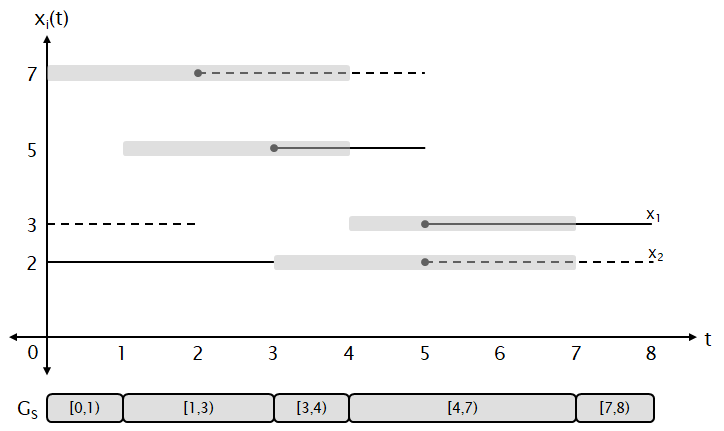
\includegraphics[scale=0.4]{canonseg.png}
	\caption{(a) Uncertainty regions and their value expressions before the segmentation. (b) The canonical segmentation of the signal and the corresponding value expressions.\label{fig:canonseg}}
\end{figure}

Given a set $L \subseteq \Sigma^*$, we define $\first(L) = \{ u[0] \st u \in L\}$.
Let $\tau_S : [0,d) \to G_S$ be a function that maps each time stamp to the interval of the canonical segmentation that it belongs to, i.e., $\tau_S(t) = [t', t'')$ where $t' \leq t < t''$ and $[t', t'') \in G_S$.
We say that two intervals $I, J \subseteq [0,d)$ with the end points $a_i < b_i$ and $a_j < b_j$ are of the same type iff the following holds: $(a_i \in I \iff a_j \in~J) \land (b_i \in I \iff b_j \in J)$.
%For $t_1, t_2 \in [0,d)$, if $\tau_S(t_1) \neq \tau_S(t_2)$, let $(J_i)_{1 \leq i \leq k}$ the (potentially empty) sequence of intervals that are strictly between $\tau_S(t_1)$ and $\tau_S(t_2)$.

Let $(S, {\hb})$ be a distributed signal of $n$ signals, $t \in [0,d)$ be a time value such that $\tau_S(t) = [t', t'')$.
Let $I \subseteq \R_{\geq 0}$ be a time interval with the end points $a < b$.
Note that timed until can be expressed using timed eventually, timed globally, and untimed until~\cite{MalerN13}.
We provide the semantics of our logic following this observation.

\scriptsize
\begin{align*}
	[S,t \models p] &=  f_p(\gamma(\tau_S(t), 1), \ldots, \gamma(\tau_S(t), n)) > 0 \\
	[S,t \models \lnot \varphi] &= \lnot [S,t \models \varphi] \\
	[S,t \models \varphi_1 \land \varphi_2] &= [S,t \models \varphi_1] \sqcap [S,t \models \varphi_2] \\
	[S,t \models \varphi_1 \until \varphi_2] &= \destutter(\{ [S,t \models \varphi_1] \until^b [S,t \models \varphi_2] \st \text{ if $t'' < d$ then $b \in \first([S,t'' \models \varphi_1 \until \varphi_2])$, otherwise $b = 0$} \}) \\
	[S,t \models \LTLf_I \varphi] &= \destutter(\{ \mathsf{E}(\textit{Pr}_1) \cdot \ldots \cdot \mathsf{E}(\textit{Pr}_M) \}) \text{ where $\textit{Pr}_i \in \mathsf{profilesBetween}(I, S, \varphi, [t',t''))$ for all $1 \leq i \leq M$} \\
	[S,t \models \LTLg_I \varphi] &= \destutter(\{ \mathsf{A}(\textit{Pr}_1) \cdot \ldots \cdot \mathsf{A}(\textit{Pr}_M) \}) \text{ where $\textit{Pr}_i \in \mathsf{profilesBetween}(I, S, \varphi, [t',t''))$ for all $1 \leq i \leq M$}
\end{align*}
\normalsize

For $s_1, s_2 \in [0,d)$, we denote by $\mathsf{profilesBetween}(I, S, \varphi, J) = \{\textit{Pr}_1, \ldots, \textit{Pr}_M\}$ the set of ``profiles'' with respect to $S$ and $\varphi$ of intervals that are a subset of $I \oplus J$ and are of the same length and type as $I$, given in an increasing order of starting points of the intervals they correspond to.
Intuitively, the profile of an interval with respect to a segmentation and a formula captures the behaviors of the given formula's satisfaction signal in that interval in terms of the value expressions of its canonical segmentation.
We formalize this below.

Let $I \subseteq [0,d)$ be an interval with the end points $a < b$.
Given $t \in [0,d)$, we let $\mathsf{end}(t, S)$ be true iff $t=d$ or $\tau_S(t) = [t, t')$ for some $t' \in [0,d)$.
Let $(H_i)_{1 \leq i \leq K}$ be a (possibly empty) sequence of intervals where $H_i = [d_i, d_{i+1}) \in G_S$ and $a < d_i < d_{i+1} < b$ for all $1 \leq i \leq K$ and $K$ is the number of intervals in $G_S$ whose endpoints are strictly between $a$ and $b$.
We denote by $Q(S, a, b)$ the concatenation of the value expressions of the intervals $H_1, \ldots, H_K$, i.e., $Q(S, a, b) = [S, d_1 \models \varphi] \cdot \ldots \cdot [S, d_K \models \varphi]$.
We define the \emph{profile} of $I \subseteq [0,d)$ with respect to $S$ and $\varphi$ as follows.

\scriptsize
	\begin{equation*} 
		\mathsf{profile}(I, S, \varphi) =
		\begin{cases}
			%		[S, a \models \varphi] &\text{if $\tau_S(a) = \tau_S(b) \land \mathsf{start}(a, S) \land \mathsf{end}(b, S)$} \\
			\pfx([S, a \models \varphi]) &\text{if $\tau_S(a) = \tau_S(b) \land \mathsf{end}(a, S)$} \\
			%		\sfx([S, a \models \varphi]) &\text{if $\tau_S(a) = \tau_S(b) \land \lnot\mathsf{start}(a, S) \land \mathsf{end}(b, S)$} \\
			\infx([S, a \models \varphi]) &\text{if $\tau_S(a) = \tau_S(b) \land \lnot\mathsf{end}(a, S)$} \\
			[S, a \models \varphi] \cdot Q(S, a, b) \cdot \first([S, b \models \varphi]) &\text{if $\tau_S(a) \neq \tau_S(b) \land \mathsf{end}(a, S) \land \mathsf{end}(b, S) \land b \in I$} \\
			[S, a \models \varphi] \cdot Q(S, a, b) &\text{if $\tau_S(a) \neq \tau_S(b) \land \mathsf{end}(a, S) \land \mathsf{end}(b, S) \land b \notin I$} \\
			[S, a \models \varphi] \cdot Q(S, a, b) \cdot \pfx([S, a \models \varphi]) &\text{if $\tau_S(a) \neq \tau_S(b) \land \mathsf{end}(a, S) \land \lnot\mathsf{end}(b, S)$} \\
			\sfx([S, a \models \varphi]) \cdot Q(S, a, b) \cdot \first([S, b \models \varphi]) &\text{if $\tau_S(a) \neq \tau_S(b) \land \lnot\mathsf{end}(a, S) \land \mathsf{end}(b, S) \land b \in I$} \\
			\sfx([S, a \models \varphi]) \cdot Q(S, a, b) &\text{if $\tau_S(a) \neq \tau_S(b) \land \lnot\mathsf{end}(a, S) \land \mathsf{end}(b, S) \land b \notin I$} \\
			\sfx([S, a \models \varphi]) \cdot Q(S, a, b) \cdot \pfx([S, b \models \varphi]) &\text{if $\tau_S(a) \neq \tau_S(b) \land \lnot\mathsf{end}(a, S) \land \lnot\mathsf{end}(b, S)$} 
		\end{cases}
	\end{equation*}
\normalsize

\begin{example}
	Recall the distributed signal  in \cref{ex:canonseg} and \cref{ex:valexpr} whose behavior is given in \cref{fig:canonseg}.
	Let $p = (x_2 > 0)$ and $q = (x_1 > 0)$ be atomic propositions
	
	First, we consider the STL formula $p \until q$.
	The value expressions of the satisfaction signals of $p$ and $q$ are the same as in \cref{fig:canonseg}b.
	We compute the values of $p \until q$ starting from the last segment $[7,8)$, which gives us $0 \mathsf{U}^0 0 = 0$.
	After handling the segment $[6,7)$ and obtain $\{ 00 \mathsf{U}^0 10, 0 \mathsf{U}^0 0 \} = \{10, 0\}$, we move to the segment $[4,6)$.
	Note that $\first(\{10, 0\}) = \{1,0\}$, therefore we compute the union of $\{10, 0\} \until^0 \{1, 10\}$ and $\{10, 0\} \until^1 \{1, 10\}$, which gives us $\{1, 10\}$.
	Continuing this way, we obtain the expressions $\{1, 01\}$ for $[2,4)$ and $\{1,0\}$ for the other two segments.
	
	Now, we consider the STL formula $\LTLeventualy_{[0,1.5]} p$.
	We show the evaluation of the value expressions corresponding to the segment $[4,6)$.
	We first need to compute the set $\mathsf{profilesBetween}([0,1.5], (x_1, x_2), p, [4,6.5))$.
	We show in \cref{fig:profiles} the intervals representing the profiles we need to compute.
	Note that the interval $[6, 7.5]$ is not included since it is not a subset of $[0, 1.5] \oplus [4,6) = [4,7.5)$.
	Let us denote by $V_t$ the set of value expression of the segment starting with $t$.
	Then, the six intervals in \cref{fig:profiles} correspond to the following profiles in order:
	\begin{enumerate}
		\item $\mathsf{Pr}_1 = \pfx(V_4) = \{1, 10, 0\}$
		\item $\mathsf{Pr}_2 = \infx(V_4) = \{1, 10, 0\}$
		\item $\mathsf{Pr}_3 = \sfx(V_4) \cdot \first(V_6) = \{100, 00\}$
		\item $\mathsf{Pr}_4 = \sfx(V_4) \cdot \pfx(V_6) = \{100, 00\}$
		\item $\mathsf{Pr}_5 = \sfx(V_4) \cdot V_6 \cdot \first(V_7) = \{1000, 000\}$
		\item $\mathsf{Pr}_6 = \sfx(V_4) \cdot V_6 \cdot \pfx(V_7)= \{1000, 000\}$
	\end{enumerate}
	Applying the bitwise-eventually operator $\mathsf{E}$ to each results in the same expressions.
	Concatenating the profiles and finally destuttering gives us the result.	
	For example, the value expression 101010101010 is in the set because each profile contains an expression equivalent to 10 after destuttering and we overapproximate the set of possible behaviors by neglecting the bookkeeping of edges.
\end{example}

\begin{figure}
	\centering
	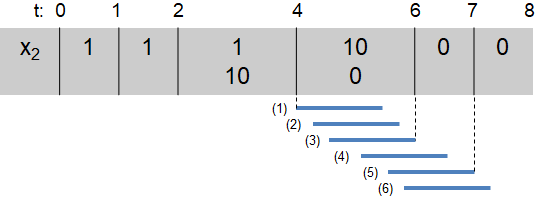
\includegraphics[scale=0.45]{profiles.png}
	\caption{The intervals representing the profiles needed to compute $\LTLeventualy_{[0,1.5]} p$ in $[4,6)$. \label{fig:profiles}}
\end{figure}